With our implementation we want to answer the following question:
\begin{quote}
  ``Given some differential characteristic, is this characteristic satisfiable?''
\end{quote}
Equivalently is there any boolean assignment within both evaluation instances such that the applied function of the hash algorithm matches the result and the bit conditions do correspond. This question was already raised in section~\ref{sec:diffchar-examples}. This is the same question stated as main difficulty for the attack of SHA-2~\cite[293]{Cry07} when trying to apply automated search.

We present various encodings and their corresponding algorithms and evaluate their performance.

\section{General architecture}
\label{sec:architecture}
%
% TODO: Introduce SAT condition as an algorithmic object (not from programmer's perspective).
%       Probably makes explanations more beautiful.
%
\subsection{Hash algorithm specification and truth table}
%
At the very beginning we specify a hash algorithm. This specification contains the elementary operations. We consider a simple hash algorithm applying the Sigma operation of the SHA-2 family consisting of XOR operations: We build a differential word of length $4$. We reuse this word three times where each time the word's values are rotated one more time to the right. The last word is the result. We get a differential characteristic of size $4\times 4$. XOR3 is now applied per bitslice.

In the implementation this hash algorithm specification is wrapped by a SAT generation unit. This unit takes a hash algorithm and creates a SAT solver equivalent for it; thus adding clauses to the SAT Solver instance instead of manipulating values in the main memory.

Every operation knows how many parameter it takes. The XOR3 operation takes three input parameters and one output parameter. It returns true if and only if the number of parameters with value true is odd. We retrieve the truth table by applying the operation one time. If the output parameters got modified for the given input, it was inconsistent and thus the entry in the truth table is false; otherwise true. This truth table is created once for every elementary operation and determines which output value is generated for the given input. Be aware that the number of evaluations is exponential to the number of variables. As such the truth table evaluation is a bottleneck in the framework. However a static implementation of the operation which directly adds the clauses can also be provided and the generation is only done once\footnote{In the Init step discussed in section~\ref{sec:nltool}.} when starting the program. Followingly we do not consider this approach as scalability threat.

Using a command line parameter \texttt{nltool} gets to know which hash algorithm to take. At this point in time, it is going to know which parameters (and their relation) are used for this hash algorithm, but not their actual values. At the same time an instance of the SAT solver is instantiated to be used later on.

The following properties are given for the elementary functions and the hash algorithm:
\begin{itemize}
  \item Any pure function using integers as arguments can be transformed into a SAT equivalent.
  \item A truth table is used exploiting exponential behavior, but this truth table generation is only run once. In a future implementation it might also run at compile time.
  \item \texttt{satstep} describes a computational unit of any scale thus allowing to combine elementary operations to advanced algebraic operations, hash algorithm rounds or even whole hash algorithms.
\end{itemize}

\subsection{Clause introduction}
\label{sec:clause-introduction}
%
Constraints to the solution of the SAT solver will be introduced in two places. The actual clauses are defined by some encoding explained in section~\ref{sec:encoding:simple-evaluation}~ff.:
\begin{itemize}
  \item For every bit condition position in the differential characteristic we provide a method such that once the bit condition value is known, the corresponding clauses (specific for this value) are added immediately.
  \item The hash algorithm defines which elementary functions are applied (for example XOR3 was applied bitslice-wise in the previous example). For all those elementary functions we generate the corresponding clauses (specific for the function).
\end{itemize}

\subsection{Structure of encodings}
\label{sec:encoding-structure}
%
A distinction of the \emph{Init} and \emph{Update} step was already defined in section~\ref{sec:nltool}. Those steps are split into several substeps in all encodings:
\begin{enumerate}
  \item Initialization
    \begin{enumerate}
      \item Detect Overlapping bits: Sometimes bit conditions are reused within a hash algorithm. For example one differential word is the rotated version of another differential word as in SHA-2 Sigma. In such a case the two bit conditions connected through rotation must be equivalent. In this step the reuse of bit conditions is detected. See section~\ref{sec:automated-search} for a more detailed discussion of overlapping bits.
      \item Introduce new bit conditions: We initialize bit condition elements in the differential characteristic without knowing their value yet.
      \item Setup encoding: For assumption-based encoding, \textbf{clauses} are added here specific for the definition of the encoding (relation between boolean variables). Request the required boolean variables from the SAT solver for each element of the differential characteristic.
      \item Apply function to bitslices: Elementary functions in \nltool{} are defined per bitslice. In this step the function is applied successively to every bitslice \textbf{adding clauses specific for the function}.
    \end{enumerate}
  \item Update BitCondition
    \begin{enumerate}
      \item Set bit condition value: Take the bit condition value and infer the corresponding \textbf{clauses or assumptions} depending on the encoding.
      \item Run SAT solver: Invoke the SAT solver and return its result as result.
    \end{enumerate}
\end{enumerate}

\newpage
\section{Approach \#1: Simple Evaluation}
\label{sec:encoding:simple-evaluation}
%
The simple evaluation approach uses 2 boolean variables per bit condition. This corresponds to one bit per evaluation instance. We apply the elementary functions to each instance (thus we define the same clauses with both sets of variables). The bit condition defines clauses which are directly derivable for the given bit condition value.

\subsection{Algorithm}
\label{sec:simple-evaluation-algorithm}
%
\begin{description}
  \item[Initialization.] Overlapping bits and the number of bit conditions are known.
    \begin{description}
      \item[Detect Overlapping Bits.] Iterate over all bit conditions and recognize overlapping bits (see section~\ref{sec:automated-search}). Store all their indices for future reference.
      \item[Introduce new bit conditions.] Define the number of bit conditions needed and their position. A bit condition gets skipped, if this is not the first reference to an overlapping bit.
      \item[Setup Encoding.] $2$ boolean variables per bit condition are requested from the SAT solver.
      \item[Apply function to bitslices.] Add all clauses which result from the function definition applied to this differential characteristic.
    \end{description}
  \item[Update BitCondition.] The values of the bit conditions are known.
    \begin{description}
      \item[Set bit condition value.] The clauses resulting from the bit condition value are added. These clauses were already discussed in the paper ``Linear propagation in Efficient Guess-and-Determine Attacks''~\cite[6]{Cry16} and repeated in Table~\ref{tab:simple-eval-clauses}. Some are them are written as XOR clauses, which are only supported by \cmsat{} 2.x and 4.x. If the SAT solver does not provide XOR clauses, you can rewrite them to CNF clauses. Appendix~\ref{appendix:cnf} lists CNF compatible equivalences for the boolean expression.
      \item[Run SAT solver.] If the SAT solver returns satisfiability as result, the differential characteristic is satisfiable.
    \end{description}
\end{description}

Algorithm~\ref{algo:apply-func-se} shows the algorithm to apply the elementary function to the bitslices and retrieve the corresponding clauses. Models are the set of input and output variables. As can be seen in the algorithm we distinguish between both instances with two boolean variables $z$ and $z^*$ and apply the same clause to both instances. The algorithm is called for every application of the elementary function to a set of arguments \texttt{sat\_args}. A clause is represented as a list like $[z_1, \neg z_2, z_3]$ equivalent to $z_1 \lor \neg z_2 \lor z_3$ in the conventional notation. Clauses are conjuncted to conjunctive normal forms.

\subsection{Discussion}
\label{sec:simple-evaluation-discussion}
%
This approach was implemented first, but has a major problem: Assuming the evaluated differential characteristic is satisfiable, a more restrictive bit condition will be used by the automated search at one position. However for the next iteration the SAT solver has to be destroyed and the configuration must be built up again. This takes a long time. We can use the fact that the Initialization step stays the same, but the Update BitCondition step is different. And so we want to use an approach which runs the Initialization step only once and the Update BitCondition is run on every search iteration.

This approach was not put into practice for the automated search and so no performance statistics are available here.

For the Update BitCondition step we are going to use SAT solver assumption. These are assignments to boolean variables which will be discarded after one run of the SAT solver without the loss of the clauses (as discussed in section~\ref{sec:satsolvers-assumptions}). Assignments are not as powerful as clauses and so the encoding has to be designed in such a way that we can use assignments to define the value of a bit condition.

\begin{algorithm}[p]
  \SetKwInOut{Input}{Input}
  \SetKwInOut{Output}{Output}
  \Input{sat\_args, function}
  \Output{a set of clauses}
  result = []\;

  \For{every possible model of elementary function}{
    \If(\tcp*[f]{that would be DNF}){model is valid}{
      continue\;
    }

    clause1 = []\;
    clause2 = []\;

    \For{every variable \textit{var} of the model}{
      \eIf{variable is true}{
        clause1.push($\neg$ sat\_args[var][$z$])\;
        clause2.push($\neg$ sat\_args[var][$z^*$])\;
      }{
        clause1.push(sat\_args[var][$z$])\;
        clause2.push(sat\_args[var][$z^*$])\;
      }
    }

    result.add(clause1)\;
    result.add(clause2)\;
  }
  return result\;
 \caption{Apply function to bitslices algorithm for Simple Evaluation.}
 \label{algo:apply-func-se}
\end{algorithm}
%
\begin{table}[p]
  \begin{center}
    \begin{tabular}{cp{5cm}cl}
      bit condition  & conjunctive normal form &
      bit condition  & conjunctive normal form \\
    \hline
      \bc{\#}        & $(z) \land (\neg z)$ &
      \bc{1}         & $(z) \land (z^*)$ \\

      \bc{0}         & $(\neg z) \land (\neg z^*)$ &
      \bc{-}         & $\neg (z \oplus z^*)$ \\

      \bc{u}         & $(z) \land (\neg z^*)$ &
      \bc{A}         & $(z)$ \\

      \bc{3}         & $(\neg z^*)$ &
      \bc{B}         & $(z \lor \neg z^*)$ \\

      \bc{n}         & $(\neg z) \land (z^*)$ &
      \bc{C}         & $(z^*)$ \\

      \bc{5}         & $(\neg z)$ &
      \bc{D}         & $(\neg z \lor z^*)$ \\

      \bc{x}         & $(z \oplus z^*)$ &
      \bc{E}         & $(z \lor z^*)$ \\

      \bc{7}         & $(\neg z \lor \neg z^*)$ &
      \bc{?}         &  \\
    \end{tabular}
    \caption[Simple Evaluation clauses]{
        Set bit condition value Simple Evaluation clauses added for a bit condition.
        A bit condition corresponds to two boolean variables $z$ and $z^*$.
    }
    \label{tab:simple-eval-clauses}
  \end{center}
\end{table}

\newpage
\section{Approach \#2: Activation literals}
\label{sec:encoding:activation-literals}
%
This approach uses the concept of \emph{activation literals}. Even though there is no explicit definition of activation literals given in prior work, the concept is used recurrently by the SAT community. One example of such is given in a paper by Niklas Een, Alan Mishchenko and Nina Amla~\cite{Sat30}.

Given a clause $c$ we introduce an activation literal $a$ to activate or deactivate this clause. Activation means that this clause becomes part of the result of the \gls{cnf}. Deactivation means that this
clause becomes true within the conjunction and therefore is not relevant for the result. $a$ is used to distinguish the (de)activation cases.

These requirements can be implemented using an implication.
\[
  a \implies b
\]

\subsection{Search with activation literals}
\label{sec:activation-literals-search}
%
To evaluate a path in the search tree a generalization of activation literals is required. We apply activation literals to sets of clauses.

Given sets of sets of clauses $S_1, S_2, S_3, \ldots, S_n$ representing nodes of a search tree, evaluate which path of this tree is satisfiable. One node is satisfiable, if all clauses of this node are satisfied. Assume a binary tree of depth 2 with $S_2$ and $S_3$ as children of $S_1$ and $S_4$ and $S_5$ as children of $S_2$ and $S_6$ and $S_7$ as children of $S_3$. The first path is given as the union of $S_1$, $S_2$ and $S_4$: $S_1 \land S_2 \land S_4$. If this path is not satisfiable, replace $S_4$ with $S_2$'s other child $S_5$ giving $S_1 \land S_2 \land S_5$. If this fails again we replace $S_2$ with $S_3$ giving us $S_1 \land S_3 \land S_6$ and $S_1 \land S_3 \land S_7$. With this concept we can evaluate any path of the tree after evaluation which clauses are part of which node.

\begin{figure}[h]
  \begin{center}
    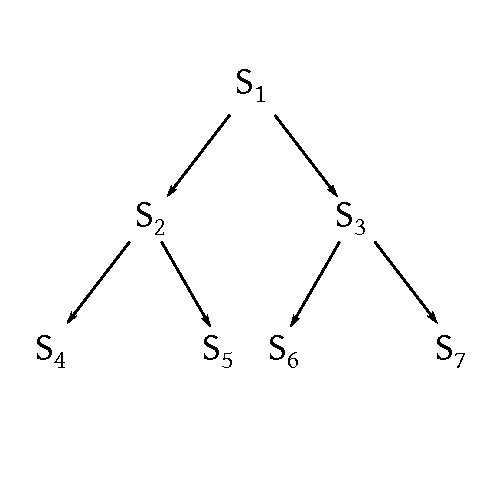
\includegraphics{img/searchtree.pdf}
    \caption{Binary search tree with sets of sets of clauses as nodes.}
    \label{fig:bintree_clauses}
  \end{center}
\end{figure}

This tree traversal can be implemented using activation literals and SAT solver assumption techniques.

If we want to evaluate the path $S_1 \land S_2 \land S_4$, we introduce a new activation literal $a_i$ for each set $S_i$ and use implication to (de)activate the clause:
%
\[
  (a_1 \implies S_1) \land (a_2 \implies S_2) \land (a_4 \implies S_4)
\]

Because each node itself is a conjunctive normal form, a set $S_i$ is the conjunction of its clauses giving us:
%
\[
  (a_1 \implies (c_1 \land c_2 \land c_3 \land \ldots)) \land
    (a_2 \implies (c_{10} \land c_{11} \land c_{12} \land \ldots)) \land
    (a_3 \implies (c_{20} \land c_{21} \land c_{22} \land \ldots)) \land
    \ldots
\]

This can be transformed to conjunctive normal form by resolving the clauses with the law of distributivity. In real-world implementations activation literals are represented as \emph{assumptions} in SAT solvers
to be able to drop their value for evaluation of the next search path (assumptions are described in section~\ref{sec:satsolvers-assumptions}).

For example the conjunctive normal form with boolean variables $v_1$ to $v_8$
%
\[
  (v_1 \lor \neg v_2) \land (\neg v_3 \lor \neg v_4 \lor v_5) \land
    (v_6 \lor v_7 \lor v_8)
\]

with activation literals $a_1$ to $a_3$
\[
  (a_1 \implies (v_1 \lor \neg v_2)) \land
    (a_2 \implies (\neg v_3 \lor \neg v_4 \lor v_5)) \land
    (a_3 \implies (v_6 \lor v_7 \lor v_8))
\]

resolved with the law of distributivity
\[
  (\neg a_1 \lor v_1 \lor \neg v_2) \land
    (\neg a_2 \lor \neg v_3 \lor \neg v_4 \lor v_5) \land
    (\neg a_3 \lor v_6 \lor v_7 \lor v_8)
\]

gives us a boolean expression in CNF.

\newpage
\subsection{Algorithm}
\label{sec:activation-literals-algorithm}
%
\begin{description}
  \item[Initialization.] Overlapping bits and the number of bit conditions are known.
    \begin{description}
      \item[Detect Overlapping Bits.] Iterate over all bit conditions and recognize overlapping bits (see section~\ref{sec:automated-search}). Store all their indices for future reference.
      \item[Introduce new bit conditions.] Define the number of bit conditions needed and their position. A bit condition gets skipped, if this is not the first reference to an overlapping bit.
      \item[Setup Encoding.] $7$ boolean variables per bit condition are requested from the SAT solver. The clauses given in Table~\ref{tab:activation-literals-clauses} are added.
      \item[Apply function to bitslices.] Add all clauses which result from the function definition applied to this differential characteristic.
    \end{description}
  \item[Update BitCondition.] The values of the bit conditions are known.
    \begin{description}
      \item[Set bit condition value.] The assumptions resulting from the bit condition value are set. They are given in Table~\ref{tab:activation-literals-assumptions}.
      \item[Run SAT solver.] If the SAT solver returns satisfiability as result, the differential characteristic is satisfiable.
    \end{description}
\end{description}

\begin{table}[p]
  \begin{center}
    \begin{tabular}{c}
      clause \\
    \hline
      $(\neg a_1 \lor z) \land (\neg a_1 \lor \neg z)$ \\
      $(\neg a_2 \lor \neg z \lor \neg z^*)$ \\
      $(\neg a_3 \lor z \lor \neg z^*)$ \\
      $(\neg a_4 \lor \neg z \lor z^*)$ \\
      $(\neg a_5 \lor z \lor z^*)$ \\
    \end{tabular}
    \caption[Activation literals clauses]%
    {Setup Encoding clauses for every element in the differential characteristic.}
    \label{tab:activation-literals-clauses}
  \end{center}
\end{table}
%
\begin{table}[p]
  \begin{center}
    \begin{tabular}{cll}
      bit condition  & Set bit condition value (assumptions) \\
    \hline
      \bc{\#}        & $a_1 = 1$ \\
      \bc{0}         & $z = 0, z^* = 0$ \\
      \bc{u}         & $z = 1, z^* = 0$ \\
      \bc{3}         & $z^* = 0$ \\
      \bc{n}         & $z = 0, z^* = 1$ \\
      \bc{5}         & $z = 0$ \\
      \bc{x}         & $a_2 = 1, a_5 = 1$ \\
      \bc{7}         & $a_2 = 1$ \\
      \bc{1}         & $z = 1, z^* = 1$ \\
      \bc{-}         & $a_3 = 1, a_4 = 1$ \\
      \bc{A}         & $z = 1$ \\
      \bc{B}         & $a_3 = 1$ \\
      \bc{C}         & $z^* = 1$ \\
      \bc{D}         & $a_4 = 1$ \\
      \bc{E}         & $a_5 = 1$ \\
      \bc{?}         &
    \end{tabular}
    \caption[Activation literals assumptions]{
        Activation literals assumptions.
        Be aware that all activation literals $a_i$ must be set to false,
        if not stated otherwise for a bit condition.
    }
    \label{tab:activation-literals-assumptions}
  \end{center}
\end{table}

\subsection{Discussion}
\label{sec:activation-literals-discussion}
%
The number of activation literals is linear to the number of nodes within the search tree. Every node represents one of sixteen possible bit conditions in worst case. However not every bit condition requires its own activation literal and corresponding clause\footnote{This approach would obviously be possible but is less efficient.}.

The bit conditions \bc{0}, \bc{u}, \bc{3}, \bc{n}, \bc{5}, \bc{1}, \bc{A}, \bc{C} and \bc{?} can directly be represented by assignments. The $5$ bit conditions \bc{\#}, \bc{7}, \bc{B}, \bc{D} and \bc{E} use the $\lor$ operator which has to be designed by explicit clauses. The bit conditions \bc{x} and \bc{-} are represented as combinations of those explicit clauses.

For one additional bit condition we need $7$ variables, $6$ clauses and $5.75$ assumptions ($21$ assumptions from the right column in Table~\ref{tab:activation-literals-assumptions} and $71$ activation literals set to false divided by $16$ bit conditions) in average. Due to the high number of assumptions we initially valued this approach as unlikely successful. The results are provided in section~\ref{sec:results};

\newpage
\section{Approach \#3: Assumption-based encodings}
\label{sec:encoding:assumption-encodings}
%
Like the activation literals approach in section~\ref{sec:encoding:activation-literals}, these approaches use assumptions to enable automated search. They do not use activation literals and only focus on efficient usage of assumptions. Three different approaches are taken which vary in the number of variables, clauses and assumptions.

\subsection{Exhaustive Encoding}
\label{sec:encoding:exhaustive}
%
The Exhaustive encoding consists of $17$ boolean variables per bit condition. Exhaustive refers to the large number of boolean variables. Each differential state gets its own assumption variable except the free bit condition~\bc{?}.

\subsubsection{Algorithm}
\label{sec:exhaustive-encoding-algorithm}
%
\begin{description}
  \item[Initialization.] Overlapping bits and the number of bit conditions are known.
    \begin{description}
      \item[Detect Overlapping Bits.] Iterate over all bit conditions and recognize overlapping bits (see section~\ref{sec:automated-search}). Store all their indices for future reference.
      \item[Introduce new bit conditions.] Define the number of bit conditions needed and their position. A bit condition gets skipped, if this is not the first reference to an overlapping bit.
      \item[Setup Encoding.] $17$ boolean variables per bit condition are requested from the SAT solver. The clauses given in Table~\ref{tab:exhaustive-encoding-clauses} are added. They correspond exactly to the expressions in Table~\ref{tab:simple-eval-clauses} but define an equivalence relation with an assumption variable $z_{\text{bit condition}}$.
      \item[Apply function to bitslices.] Add all clauses which result from the function definition applied to this differential characteristic.
    \end{description}
  \item[Update BitCondition.] The values of the bit conditions are known.
    \begin{description}
      \item[Set bit condition value.] Given a bit condition $T$, the corresponding assumption $z_T$ is set to true. For the free variable nothing is set true.
      \item[Run SAT solver.] If the SAT solver returns satisfiability as result, the differential characteristic is satisfiable.
    \end{description}
\end{description}

\begin{table}[t]
  \begin{center}
    \begin{tabular}{cp{5cm}cl}
      $z_\#$ & $= \neg z_\#$ &
      $z_1$  & $= z \land z^*$ \\

      $z_0$  & $= \neg z \land \neg z^*$ &
      $z_-$  & $= \neg(z \oplus z^*)$ \\

      $z_u$  & $= z \land \neg z^*$ &
      $z_A$  & $= z$ \\

      $z_3$  & $= \neg z^*$ &
      $z_B$  & $= z \lor \neg z^*$ \\

      $z_n$  & $= \neg z \land z^*$ &
      $z_C$  & $= z^*$ \\

      $z_5$  & $= \neg z$ &
      $z_D$  & $= \neg z \lor z^*$ \\

      $z_X$  & $= z \oplus z^*$ &
      $z_E$  & $= z \lor z^*$ \\

      $z_7$  & $= \neg z \lor \neg z^*$ &
             & \\
    \end{tabular}
    \caption{Exhaustive encoding clauses.}
    \label{tab:exhaustive-encoding-clauses}
  \end{center}
\end{table}

\subsubsection{Discussion}
\label{sec:exhaustive-discussion}
%
For this encoding obviously some reductions can be applied if one bit condition is a superset of another one (as can be seen in the lattice of Figure~\ref{fig:bitconditions-lattice}). Those reductions have been applied in the following encodings. Because this encoding has an extraordinary high number of variables, we assume that this encoding will not perform good in any case. Because no implementation was provided, no statistics are available.

\newpage
\subsection{Reduced Encoding}
\label{sec:encoding:reduced-encoding}
%
The following approach was initially proposed by Martin Schläffer. It takes $9$ variables for each bit condition denoted as $z, z^*, z_A, z_B, z_C, z_D, z_E, z_x$ and $z_1$.

\subsubsection{Algorithm}
\label{sec:reduced-encoding-algorithm}
%
\begin{description}
  \item[Initialization.] Overlapping bits and the number of bit conditions are known.
    \begin{description}
      \item[Detect Overlapping Bits.] Iterate over all bit conditions and recognize overlapping bits (see section~\ref{sec:automated-search}). Store all their indices for future reference.
      \item[Introduce new bit conditions.] Define the number of bit conditions needed and their position. A bit condition gets skipped, if this is not the first reference to an overlapping bit.
      \item[Setup Encoding.] $9$ boolean variables per bit condition are requested from the SAT solver. The clauses given in Table~\ref{tab:reduced-encoding-clauses} are added.
      \item[Apply function to bitslices.] Add all clauses which result from the function definition applied to this differential characteristic.
    \end{description}
  \item[Update BitCondition.] The values of the bit conditions are known.
    \begin{description}
      \item[Set bit condition value.] The assumptions resulting from the bit condition value are set. They are given in Table~\ref{tab:reduced-encoding-assumptions}.
      \item[Run SAT solver.] If the SAT solver returns satisfiability as result, the differential characteristic is satisfiable.
    \end{description}
\end{description}

\begin{table}[h]
  \begin{center}
    \begin{tabular}{ll}
      $z_A$ & $= z_1$ \\
      $z_B$ & $= z_1 \lor \neg z_1^*$ \\
      $z_C$ & $= z^*$ \\
      $z_D$ & $= \neg z \lor z^*$ \\
      $z_E$ & $= z \lor z^*$ \\
      $z_X$ & $= z \oplus z^*$ \\
      $z_1$ & $= z \land z^*$
    \end{tabular}
    \caption{Reduced encoding clauses.}
    \label{tab:reduced-encoding-clauses}
  \end{center}
\end{table}
%
\begin{table}[t]
  \begin{center}
    \begin{tabular}{cll}
      bit condition  & Set bit condition value \\
    \hline
      \bc{\#}        & $z_1 = 1, z_x = 1$ \\
      \bc{0}         & $z_A = 0, z_C = 0$ \\
      \bc{u}         & $z_A = 1, z_C = 0$ \\
      \bc{3}         & $z_C = 0$ \\
      \bc{n}         & $z_A = 0, z_C = 0$ \\
      \bc{5}         & $z_A = 0$ \\
      \bc{x}         & $z_X = 1$ \\
      \bc{7}         & $z_1 = 0$ \\
      \bc{1}         & $z_1 = 1$ \\
      \bc{-}         & $z_X = 0$ \\
      \bc{A}         & $z_A = 1$ \\
      \bc{B}         & $z_B = 1$ \\
      \bc{C}         & $z_C = 1$ \\
      \bc{D}         & $z_D = 1$ \\
      \bc{E}         & $z_E = 1$ \\
      \bc{?}         & 
    \end{tabular}
    \caption{Assumptions for the Reduced encoding.}
    \label{tab:reduced-encoding-assumptions}
  \end{center}
\end{table}

\subsubsection{Discussion}
\label{sec:reduced-encoding-discussion}
%
One additional bit condition requires $9$ boolean variables, $20$ clauses\footnote{Table~\ref{tab:reduced-encoding-clauses} transformed to CNF using the equivalences of Appendix~\ref{appendix:cnf} gives us 20 clauses.} and $1.1875$ assumptions in average\footnote{19 assumptions if every bit condition occurs once divided by 16 possible bit conditions.}.
This encoding provides a nice tradeoff between a small number of clauses and variables and was the first stable implementation to evaluate differential characteristics with a SAT solver.

\newpage
\subsection{Differential state encoding}
\label{sec:encoding:dse}
%
\subsubsection{Algorithm}
\label{sec:encoding:dse-algorithm}
%
The 4 variables are denoted as $z_0, z_n, z_u$ and $z_1$. They exactly correspond to the cases $(0, 0), (0, 1), (1, 0)$ and $(1, 1)$ for bits in the evaluation instances. We require that only one of the cases is met.

This encoding differs from the other encoding in a sense that the Initialization is very much different and takes up more time whereas the small number of variables is expected to outweigh this performance problem in the Initialization.
%
\begin{description}
  \item[Initialization.] Overlapping bits and the number of bit conditions are known.
    \begin{description}
      \item[Detect Overlapping Bits.] Iterate over all bit conditions and store overlapping bit conditions.
      \item[Introduce new bit conditions.] Define the number of bit conditions needed and their position. A bit condition gets skipped, if this is not the first reference to an overlapping bit.
      \item[Setup Encoding.] $4$ boolean variables per bit condition are requested from the SAT solver. We ensure that only one the four boolean variables becomes true. Table~\ref{tab:dse-clauses} lists the clauses.
      \item[Apply function to bitslices.] See Algorithm~\ref{algo:dse-function}.
    \end{description}
  \item[Update BitCondition.] The values of the bit conditions are known.
    \begin{description}
      \item[Set bit condition value.] The assumptions resulting from the bit condition value are set. They are given in Table~\ref{tab:dse-assumptions}.
      \item[Run SAT solver.] If the SAT solver returns satisfiability as result, the differential characteristic is satisfiable.
    \end{description}
\end{description}

\begin{table}[p]
  \begin{center}
    \begin{alignat*}{4}
      (z_A      & \oplus    z_B & & \oplus    z_C & & \oplus    z_D & & )\, \land \\
      (z_A      & \lor \neg z_B & & \lor \neg z_C & & \lor \neg z_D & & )\, \land \\
      (\neg z_A & \lor      z_B & & \lor \neg z_C & & \lor \neg z_D & & )\, \land \\
      (\neg z_A & \lor \neg z_B & & \lor      z_C & & \lor \neg z_D & & )\, \land \\
      (\neg z_A & \lor \neg z_B)& & \lor \neg z_C & & \lor      z_D & & ) \\
    \end{alignat*}
    \caption{Setup Encoding clauses to ensure only one variable is set to true (with 1 XOR clauses) (can be written as 7 CNF clauses).}
    \label{tab:dse-clauses}
  \end{center}
\end{table}
%
\begin{table}[t]
  \begin{center}
    \begin{tabular}{cll}
      bit condition  & Set bit condition value \\
    \hline
      \bc{\#}        & $z_A = 0, z_B = 0, z_C = 0, z_D = 0$ \\
      \bc{0}         & $z_A = 1$ \\
      \bc{u}         & $z_C = 1$ \\
      \bc{3}         & $z_B = 0, z_D = 0$ \\
      \bc{n}         & $z_B = 1$ \\
      \bc{5}         & $z_C = 0, z_D = 0$ \\
      \bc{x}         & $z_A = 0, z_D = 0$ \\
      \bc{7}         & $z_D = 0$ \\
      \bc{1}         & $z_D = 1$ \\
      \bc{-}         & $z_B = 0, z_C = 0$ \\
      \bc{A}         & $z_A = 0, z_D = 0$ \\
      \bc{B}         & $z_B = 0$ \\
      \bc{C}         & $z_A = 0, z_C = 0$ \\
      \bc{D}         & $z_C = 0$ \\
      \bc{E}         & $z_A = 0$ \\
      \bc{?}         & 
    \end{tabular}
    \caption{Assumptions for the Differential State encoding.}
    \label{tab:dse-assumptions}
  \end{center}
\end{table}
%
\begin{algorithm}[p]
  \SetKwInOut{Input}{Input}
  \SetKwInOut{Output}{Output}
  \Input{sat\_args, function}
  \Output{a set of clauses}
  result = []\;

  \For{every possible model $i$ of function}{
    \For{every possible model $j$ of function}{
      \If{model $i$ is valid and model $j$ is valid}{
        continue\;
      }

      clause = []\;

      \For{every variable \textit{var} of any model}{
        \Switch{bit condition corresponding $i[\textit{var}]$ and $j[\textit{var}]$}{
          \Case{0}{clause.push($\neg$ sat\_args[\textit{var}][$z_0$])\;}
          \Case{n}{clause.push($\neg$ sat\_args[\textit{var}][$z_n$])\;}
          \Case{u}{clause.push($\neg$ sat\_args[\textit{var}][$z_u$])\;}
          \Case{1}{clause.push($\neg$ sat\_args[\textit{var}][$z_1$])\;}
        }
      }

      result.push(clause)\;
    }
  }

  return result\;
 \caption[Apply function to bitslices algorithm for DSE]%
   {Apply function to bitslices algorithm for DSE. Recognize the nested
   for loop over models indicating a much worse scalability in the Initialize step.}
 \label{algo:dse-function}
\end{algorithm}


\subsubsection{Discussion}
\label{sec:dse-discussion}
%
This approach was meant to radically reduce the number of variables to achieve better performance as response to Reduced Encoding. As it turns out a small number of variables is not the important speedup measure for CNFs.

One additional bit condition requires $4$ boolean variables, $4$ or $7$ clauses and $1.5$ assumptions in average. The open question is which one is worse: a high number of clauses or a high number of variables. A high number of variables might segment the search space for the SAT solver which leads to fast evaluation. This question was not discussed thoroughly by analyzing the SAT solver, but the results in section~\ref{sec:results} provide an indicator.
